\documentclass[11pt,a4paper]{article}

\usepackage{Act}
\usepackage{listings,tcolorbox}
\begin{document}
\newcommand{\ModeExercice}{
% Traduction des noms pour le package exercise
\renewcommand{\ExerciseName}{Exercice}
}

\newcommand{\ModeActivite}{
% Traduction des noms pour le package exercise
\renewcommand{\ExerciseName}{Activité}
}
% Réglages de la mise en forme des exercices 
\renewcommand{\ExerciseHeaderTitle}{\ExerciseTitle}
\renewcommand{\ExerciseHeaderOrigin}{\ExerciseOrigin}
% Un : sépare le numéro de l'exerice de son titre ... si le titre existe. On utilise Origine pour placer les pictogrammes en fin de ligne
\renewcommand{\ExerciseHeader}{\ding{113} \textbf{\sffamily{\ExerciseName \ \ExerciseHeaderNB}} \ifthenelse{\equal{\ExerciseTitle}{\empty}}{}{:} \textit{\ExerciseHeaderTitle} \hfill \ExerciseHeaderOrigin}


%QCM de NSI \QNSI{Question}{R1}{R2}{R3}{R4}
\newcommand{\QNSI}[5]{
#1
\begin{enumerate}[label=\alph{enumi})]
\item #2
\item #3
\item #4
\item #5
\end{enumerate}
}



\definecolor{grispale}{gray}{0.95}
\newcommand{\htmlmode}{\lstset{language=html,numbers=left, tabsize=2, frame=single, breaklines=true, keywordstyle=\ttfamily, basicstyle=\small,
   numberstyle=\tiny\ttfamily, framexleftmargin=0mm, backgroundcolor=\color{grispale}, xleftmargin=12mm,showstringspaces=false}}
\newcommand{\pythonmode}{\lstset{language=python,numbers=left, tabsize=4, frame=single, breaklines=true, keywordstyle=\ttfamily, basicstyle=\small,
   numberstyle=\tiny\ttfamily, framexleftmargin=0mm, backgroundcolor=\color{grispale}, xleftmargin=12mm, showstringspaces=false}}
\newcommand{\bashmode}{\lstset{language=bash,numbers=left, tabsize=2, frame=single, breaklines=true, basicstyle=\ttfamily,
   numberstyle=\tiny\ttfamily, framexleftmargin=0mm, backgroundcolor=\color{grispale}, xleftmargin=12mm, showstringspaces=false}}
\newcommand{\exomode}{\lstset{language=python,numbers=left, tabsize=2, frame=single, breaklines=true, basicstyle=\ttfamily,
   numberstyle=\tiny\ttfamily, framexleftmargin=13mm, xleftmargin=12mm, basicstyle=\small, showstringspaces=false}}
   
   
  \lstset{%
        inputencoding=utf8,
        extendedchars=true,
        literate=%
        {é}{{\'{e}}}1
        {è}{{\`{e}}}1
        {ê}{{\^{e}}}1
        {ë}{{\¨{e}}}1
        {É}{{\'{E}}}1
        {Ê}{{\^{E}}}1
        {û}{{\^{u}}}1
        {ù}{{\`{u}}}1
        {ú}{{\'{u}}}1
        {â}{{\^{a}}}1
        {à}{{\`{a}}}1
        {á}{{\'{a}}}1
        {ã}{{\~{a}}}1
        {Á}{{\'{A}}}1
        {Â}{{\^{A}}}1
        {Ã}{{\~{A}}}1
        {ç}{{\c{c}}}1
        {Ç}{{\c{C}}}1
        {õ}{{\~{o}}}1
        {ó}{{\'{o}}}1
        {ô}{{\^{o}}}1
        {Õ}{{\~{O}}}1
        {Ó}{{\'{O}}}1
        {Ô}{{\^{O}}}1
        {î}{{\^{i}}}1
        {Î}{{\^{I}}}1
        {í}{{\'{i}}}1
        {Í}{{\~{Í}}}1
}

%tei pour placer les images
%tei{nom de l’image}{échelle de l’image}{sens}{texte a positionner}
%sens ="1" (droite) ou "2" (gauche)
\newlength{\ltxt}
\newcommand{\tei}[4]{
\setlength{\ltxt}{\linewidth}
\setbox0=\hbox{\includegraphics[scale=#2]{#1}}
\addtolength{\ltxt}{-\wd0}
\addtolength{\ltxt}{-10pt}
\ifthenelse{\equal{#3}{1}}{
\begin{minipage}{\wd0}
\includegraphics[scale=#2]{#1}
\end{minipage}
\hfill
\begin{minipage}{\ltxt}
#4
\end{minipage}
}{
\begin{minipage}{\ltxt}
#4
\end{minipage}
\hfill
\begin{minipage}{\wd0}
\includegraphics[scale=#2]{#1}
\end{minipage}
}
}

%Juxtaposition d'une image pspciture et de texte 
%#1: = code pstricks de l'image
%#2: largeur de l'image
%#3: hauteur de l'image
%#4: Texte à écrire
\newcommand{\ptp}[4]{
\setlength{\ltxt}{\linewidth}
\addtolength{\ltxt}{-#2 cm}
\addtolength{\ltxt}{-0.1 cm}
\begin{minipage}[b][#3 cm][t]{\ltxt}
#4
\end{minipage}\hfill
\begin{minipage}[b][#3 cm][c]{#2 cm}
#1
\end{minipage}\par
}



%Macros pour les graphiques
\psset{linewidth=0.5\pslinewidth,PointSymbol=x}
\setlength{\fboxrule}{0.5pt}
\newcounter{tempangle}

%Marque la longueur du segment d'extrémité  #1 et  #2 avec la valeur #3, #4 est la distance par rapport au segment (en %age de la valeur de celui ci) et #5 l'orientation du marquage : +90 ou -90
\newcommand{\afflong}[5]{
\pstRotation[RotAngle=#4,PointSymbol=none,PointName=none]{#1}{#2}[X] 
\pstHomO[PointSymbol=none,PointName=none,HomCoef=#5]{#1}{X}[Y]
\pstTranslation[PointSymbol=none,PointName=none]{#1}{#2}{Y}[Z]
 \ncline{|<->|,linewidth=0.25\pslinewidth}{Y}{Z} \ncput*[nrot=:U]{\footnotesize{#3}}
}
\newcommand{\afflongb}[3]{
\ncline{|<->|,linewidth=0}{#1}{#2} \naput*[nrot=:U]{\footnotesize{#3}}
}

%Construis le point #4 situé à #2 cm du point #1 avant un angle #3 par rapport à l'horizontale. #5 = liste de paramètre
\newcommand{\lsegment}[5]{\pstGeonode[PointSymbol=none,PointName=none](0,0){O'}(#2,0){I'} \pstTranslation[PointSymbol=none,PointName=none]{O'}{I'}{#1}[J'] \pstRotation[RotAngle=#3,PointSymbol=x,#5]{#1}{J'}[#4]}
\newcommand{\tsegment}[5]{\pstGeonode[PointSymbol=none,PointName=none](0,0){O'}(#2,0){I'} \pstTranslation[PointSymbol=none,PointName=none]{O'}{I'}{#1}[J'] \pstRotation[RotAngle=#3,PointSymbol=x,#5]{#1}{J'}[#4] \pstLineAB{#4}{#1}}

%Construis le point #4 situé à #3 cm du point #1 et faisant un angle de  90° avec la droite (#1,#2) #5 = liste de paramètre
\newcommand{\psegment}[5]{
\pstGeonode[PointSymbol=none,PointName=none](0,0){O'}(#3,0){I'}
 \pstTranslation[PointSymbol=none,PointName=none]{O'}{I'}{#1}[J']
 \pstInterLC[PointSymbol=none,PointName=none]{#1}{#2}{#1}{J'}{M1}{M2} \pstRotation[RotAngle=-90,PointSymbol=x,#5]{#1}{M1}[#4]
  }
  
%Construis le point #4 situé à #3 cm du point #1 et faisant un angle de  #5° avec la droite (#1,#2) #6 = liste de paramètre
\newcommand{\mlogo}[6]{
\pstGeonode[PointSymbol=none,PointName=none](0,0){O'}(#3,0){I'}
 \pstTranslation[PointSymbol=none,PointName=none]{O'}{I'}{#1}[J']
 \pstInterLC[PointSymbol=none,PointName=none]{#1}{#2}{#1}{J'}{M1}{M2} \pstRotation[RotAngle=#5,PointSymbol=x,#6]{#1}{M2}[#4]
  }

% Construis un triangle avec #1=liste des 3 sommets séparés par des virgules, #2=liste des 3 longueurs séparés par des virgules, #3 et #4 : paramètre d'affichage des 2e et 3 points et #5 : inclinaison par rapport à l'horizontale
%autre macro identique mais sans tracer les segments joignant les sommets
\noexpandarg
\newcommand{\Triangleccc}[5]{
\StrBefore{#1}{,}[\pointA]
\StrBetween[1,2]{#1}{,}{,}[\pointB]
\StrBehind[2]{#1}{,}[\pointC]
\StrBefore{#2}{,}[\coteA]
\StrBetween[1,2]{#2}{,}{,}[\coteB]
\StrBehind[2]{#2}{,}[\coteC]
\tsegment{\pointA}{\coteA}{#5}{\pointB}{#3} 
\lsegment{\pointA}{\coteB}{0}{Z1}{PointSymbol=none, PointName=none}
\lsegment{\pointB}{\coteC}{0}{Z2}{PointSymbol=none, PointName=none}
\pstInterCC{\pointA}{Z1}{\pointB}{Z2}{\pointC}{Z3} 
\pstLineAB{\pointA}{\pointC} \pstLineAB{\pointB}{\pointC}
\pstSymO[PointName=\pointC,#4]{C}{C}[C]
}
\noexpandarg
\newcommand{\TrianglecccP}[5]{
\StrBefore{#1}{,}[\pointA]
\StrBetween[1,2]{#1}{,}{,}[\pointB]
\StrBehind[2]{#1}{,}[\pointC]
\StrBefore{#2}{,}[\coteA]
\StrBetween[1,2]{#2}{,}{,}[\coteB]
\StrBehind[2]{#2}{,}[\coteC]
\tsegment{\pointA}{\coteA}{#5}{\pointB}{#3} 
\lsegment{\pointA}{\coteB}{0}{Z1}{PointSymbol=none, PointName=none}
\lsegment{\pointB}{\coteC}{0}{Z2}{PointSymbol=none, PointName=none}
\pstInterCC[PointNameB=none,PointSymbolB=none,#4]{\pointA}{Z1}{\pointB}{Z2}{\pointC}{Z1} 
}


% Construis un triangle avec #1=liste des 3 sommets séparés par des virgules, #2=liste formée de 2 longueurs et d'un angle séparés par des virgules, #3 et #4 : paramètre d'affichage des 2e et 3 points et #5 : inclinaison par rapport à l'horizontale
%autre macro identique mais sans tracer les segments joignant les sommets
\newcommand{\Trianglecca}[5]{
\StrBefore{#1}{,}[\pointA]
\StrBetween[1,2]{#1}{,}{,}[\pointB]
\StrBehind[2]{#1}{,}[\pointC]
\StrBefore{#2}{,}[\coteA]
\StrBetween[1,2]{#2}{,}{,}[\coteB]
\StrBehind[2]{#2}{,}[\angleA]
\tsegment{\pointA}{\coteA}{#5}{\pointB}{#3} 
\setcounter{tempangle}{#5}
\addtocounter{tempangle}{\angleA}
\tsegment{\pointA}{\coteB}{\thetempangle}{\pointC}{#4}
\pstLineAB{\pointB}{\pointC}
}
\newcommand{\TriangleccaP}[5]{
\StrBefore{#1}{,}[\pointA]
\StrBetween[1,2]{#1}{,}{,}[\pointB]
\StrBehind[2]{#1}{,}[\pointC]
\StrBefore{#2}{,}[\coteA]
\StrBetween[1,2]{#2}{,}{,}[\coteB]
\StrBehind[2]{#2}{,}[\angleA]
\lsegment{\pointA}{\coteA}{#5}{\pointB}{#3} 
\setcounter{tempangle}{#5}
\addtocounter{tempangle}{\angleA}
\lsegment{\pointA}{\coteB}{\thetempangle}{\pointC}{#4}
}

% Construis un triangle avec #1=liste des 3 sommets séparés par des virgules, #2=liste formée de 1 longueurs et de deux angle séparés par des virgules, #3 et #4 : paramètre d'affichage des 2e et 3 points et #5 : inclinaison par rapport à l'horizontale
%autre macro identique mais sans tracer les segments joignant les sommets
\newcommand{\Trianglecaa}[5]{
\StrBefore{#1}{,}[\pointA]
\StrBetween[1,2]{#1}{,}{,}[\pointB]
\StrBehind[2]{#1}{,}[\pointC]
\StrBefore{#2}{,}[\coteA]
\StrBetween[1,2]{#2}{,}{,}[\angleA]
\StrBehind[2]{#2}{,}[\angleB]
\tsegment{\pointA}{\coteA}{#5}{\pointB}{#3} 
\setcounter{tempangle}{#5}
\addtocounter{tempangle}{\angleA}
\lsegment{\pointA}{1}{\thetempangle}{Z1}{PointSymbol=none, PointName=none}
\setcounter{tempangle}{#5}
\addtocounter{tempangle}{180}
\addtocounter{tempangle}{-\angleB}
\lsegment{\pointB}{1}{\thetempangle}{Z2}{PointSymbol=none, PointName=none}
\pstInterLL[#4]{\pointA}{Z1}{\pointB}{Z2}{\pointC}
\pstLineAB{\pointA}{\pointC}
\pstLineAB{\pointB}{\pointC}
}
\newcommand{\TrianglecaaP}[5]{
\StrBefore{#1}{,}[\pointA]
\StrBetween[1,2]{#1}{,}{,}[\pointB]
\StrBehind[2]{#1}{,}[\pointC]
\StrBefore{#2}{,}[\coteA]
\StrBetween[1,2]{#2}{,}{,}[\angleA]
\StrBehind[2]{#2}{,}[\angleB]
\lsegment{\pointA}{\coteA}{#5}{\pointB}{#3} 
\setcounter{tempangle}{#5}
\addtocounter{tempangle}{\angleA}
\lsegment{\pointA}{1}{\thetempangle}{Z1}{PointSymbol=none, PointName=none}
\setcounter{tempangle}{#5}
\addtocounter{tempangle}{180}
\addtocounter{tempangle}{-\angleB}
\lsegment{\pointB}{1}{\thetempangle}{Z2}{PointSymbol=none, PointName=none}
\pstInterLL[#4]{\pointA}{Z1}{\pointB}{Z2}{\pointC}
}

%Construction d'un cercle de centre #1 et de rayon #2 (en cm)
\newcommand{\Cercle}[2]{
\lsegment{#1}{#2}{0}{Z1}{PointSymbol=none, PointName=none}
\pstCircleOA{#1}{Z1}
}

%construction d'un parallélogramme #1 = liste des sommets, #2 = liste contenant les longueurs de 2 côtés consécutifs et leurs angles;  #3, #4 et #5 : paramètre d'affichage des sommets #6 inclinaison par rapport à l'horizontale 
% meme macro sans le tracé des segements
\newcommand{\Para}[6]{
\StrBefore{#1}{,}[\pointA]
\StrBetween[1,2]{#1}{,}{,}[\pointB]
\StrBetween[2,3]{#1}{,}{,}[\pointC]
\StrBehind[3]{#1}{,}[\pointD]
\StrBefore{#2}{,}[\longueur]
\StrBetween[1,2]{#2}{,}{,}[\largeur]
\StrBehind[2]{#2}{,}[\angle]
\tsegment{\pointA}{\longueur}{#6}{\pointB}{#3} 
\setcounter{tempangle}{#6}
\addtocounter{tempangle}{\angle}
\tsegment{\pointA}{\largeur}{\thetempangle}{\pointD}{#5}
\pstMiddleAB[PointName=none,PointSymbol=none]{\pointB}{\pointD}{Z1}
\pstSymO[#4]{Z1}{\pointA}[\pointC]
\pstLineAB{\pointB}{\pointC}
\pstLineAB{\pointC}{\pointD}
}
\newcommand{\ParaP}[6]{
\StrBefore{#1}{,}[\pointA]
\StrBetween[1,2]{#1}{,}{,}[\pointB]
\StrBetween[2,3]{#1}{,}{,}[\pointC]
\StrBehind[3]{#1}{,}[\pointD]
\StrBefore{#2}{,}[\longueur]
\StrBetween[1,2]{#2}{,}{,}[\largeur]
\StrBehind[2]{#2}{,}[\angle]
\lsegment{\pointA}{\longueur}{#6}{\pointB}{#3} 
\setcounter{tempangle}{#6}
\addtocounter{tempangle}{\angle}
\lsegment{\pointA}{\largeur}{\thetempangle}{\pointD}{#5}
\pstMiddleAB[PointName=none,PointSymbol=none]{\pointB}{\pointD}{Z1}
\pstSymO[#4]{Z1}{\pointA}[\pointC]
}


%construction d'un cerf-volant #1 = liste des sommets, #2 = liste contenant les longueurs de 2 côtés consécutifs et leurs angles;  #3, #4 et #5 : paramètre d'affichage des sommets #6 inclinaison par rapport à l'horizontale 
% meme macro sans le tracé des segements
\newcommand{\CerfVolant}[6]{
\StrBefore{#1}{,}[\pointA]
\StrBetween[1,2]{#1}{,}{,}[\pointB]
\StrBetween[2,3]{#1}{,}{,}[\pointC]
\StrBehind[3]{#1}{,}[\pointD]
\StrBefore{#2}{,}[\longueur]
\StrBetween[1,2]{#2}{,}{,}[\largeur]
\StrBehind[2]{#2}{,}[\angle]
\tsegment{\pointA}{\longueur}{#6}{\pointB}{#3} 
\setcounter{tempangle}{#6}
\addtocounter{tempangle}{\angle}
\tsegment{\pointA}{\largeur}{\thetempangle}{\pointD}{#5}
\pstOrtSym[#4]{\pointB}{\pointD}{\pointA}[\pointC]
\pstLineAB{\pointB}{\pointC}
\pstLineAB{\pointC}{\pointD}
}

%construction d'un quadrilatère quelconque #1 = liste des sommets, #2 = liste contenant les longueurs des 4 côtés et l'angle entre 2 cotés consécutifs  #3, #4 et #5 : paramètre d'affichage des sommets #6 inclinaison par rapport à l'horizontale 
% meme macro sans le tracé des segements
\newcommand{\Quadri}[6]{
\StrBefore{#1}{,}[\pointA]
\StrBetween[1,2]{#1}{,}{,}[\pointB]
\StrBetween[2,3]{#1}{,}{,}[\pointC]
\StrBehind[3]{#1}{,}[\pointD]
\StrBefore{#2}{,}[\coteA]
\StrBetween[1,2]{#2}{,}{,}[\coteB]
\StrBetween[2,3]{#2}{,}{,}[\coteC]
\StrBetween[3,4]{#2}{,}{,}[\coteD]
\StrBehind[4]{#2}{,}[\angle]
\tsegment{\pointA}{\coteA}{#6}{\pointB}{#3} 
\setcounter{tempangle}{#6}
\addtocounter{tempangle}{\angle}
\tsegment{\pointA}{\coteD}{\thetempangle}{\pointD}{#5}
\lsegment{\pointB}{\coteB}{0}{Z1}{PointSymbol=none, PointName=none}
\lsegment{\pointD}{\coteC}{0}{Z2}{PointSymbol=none, PointName=none}
\pstInterCC[PointNameA=none,PointSymbolA=none,#4]{\pointB}{Z1}{\pointD}{Z2}{Z3}{\pointC} 
\pstLineAB{\pointB}{\pointC}
\pstLineAB{\pointC}{\pointD}
}


% Définition des colonnes centrées ou à droite pour tabularx
\newcolumntype{Y}{>{\centering\arraybackslash}X}
\newcolumntype{Z}{>{\flushright\arraybackslash}X}

%Les pointillés à remplir par les élèves
\newcommand{\po}[1]{\makebox[#1 cm]{\dotfill}}
\newcommand{\lpo}[1][3]{%
\multido{}{#1}{\makebox[\linewidth]{\dotfill}
}}

%Liste des pictogrammes utilisés sur la fiche d'exercice ou d'activités
\newcommand{\bombe}{\faBomb}
\newcommand{\livre}{\faBook}
\newcommand{\calculatrice}{\faCalculator}
\newcommand{\oral}{\faCommentO}
\newcommand{\surfeuille}{\faEdit}
\newcommand{\ordinateur}{\faLaptop}
\newcommand{\ordi}{\faDesktop}
\newcommand{\ciseaux}{\faScissors}
\newcommand{\danger}{\faExclamationTriangle}
\newcommand{\out}{\faSignOut}
\newcommand{\cadeau}{\faGift}
\newcommand{\flash}{\faBolt}
\newcommand{\lumiere}{\faLightbulb}
\newcommand{\compas}{\dsmathematical}
\newcommand{\calcullitteral}{\faTimesCircleO}
\newcommand{\raisonnement}{\faCogs}
\newcommand{\recherche}{\faSearch}
\newcommand{\rappel}{\faHistory}
\newcommand{\video}{\faFilm}
\newcommand{\capacite}{\faPuzzlePiece}
\newcommand{\aide}{\faLifeRing}
\newcommand{\loin}{\faExternalLink}
\newcommand{\groupe}{\faUsers}
\newcommand{\bac}{\faGraduationCap}
\newcommand{\histoire}{\faUniversity}
\newcommand{\coeur}{\faSave}
\newcommand{\python}{\faPython}
\newcommand{\os}{\faMicrochip}
\newcommand{\rd}{\faCubes}
\newcommand{\data}{\faColumns}
\newcommand{\web}{\faCode}
\newcommand{\prog}{\faFile}
\newcommand{\algo}{\faCogs}
\newcommand{\important}{\faExclamationCircle}
\newcommand{\maths}{\faTimesCircle}
% Traitement des données en tables
\newcommand{\tables}{\faColumns}
% Types construits
\newcommand{\construits}{\faCubes}
% Type et valeurs de base
\newcommand{\debase}{{\footnotesize \faCube}}
% Systèmes d'exploitation
\newcommand{\linux}{\faLinux}
\newcommand{\sd}{\faProjectDiagram}
\newcommand{\bd}{\faDatabase}

%Les ensembles de nombres
\renewcommand{\N}{\mathbb{N}}
\newcommand{\D}{\mathbb{D}}
\newcommand{\Z}{\mathbb{Z}}
\newcommand{\Q}{\mathbb{Q}}
\newcommand{\R}{\mathbb{R}}
\newcommand{\C}{\mathbb{C}}

%Ecriture des vecteurs
\newcommand{\vect}[1]{\vbox{\halign{##\cr 
  \tiny\rightarrowfill\cr\noalign{\nointerlineskip\vskip1pt} 
  $#1\mskip2mu$\cr}}}


%Compteur activités/exos et question et mise en forme titre et questions
\newcounter{numact}
\setcounter{numact}{1}
\newcounter{numseance}
\setcounter{numseance}{1}
\newcounter{numexo}
\setcounter{numexo}{0}
\newcounter{numprojet}
\setcounter{numprojet}{0}
\newcounter{numquestion}
\newcommand{\espace}[1]{\rule[-1ex]{0pt}{#1 cm}}
\newcommand{\Quest}[3]{
\addtocounter{numquestion}{1}
\begin{tabularx}{\textwidth}{X|m{1cm}|}
\cline{2-2}
\textbf{\sffamily{\alph{numquestion})}} #1 & \dots / #2 \\
\hline 
\multicolumn{2}{|l|}{\espace{#3}} \\
\hline
\end{tabularx}
}
\newcommand{\QuestR}[3]{
\addtocounter{numquestion}{1}
\begin{tabularx}{\textwidth}{X|m{1cm}|}
\cline{2-2}
\textbf{\sffamily{\alph{numquestion})}} #1 & \dots / #2 \\
\hline 
\multicolumn{2}{|l|}{\cor{#3}} \\
\hline
\end{tabularx}
}
\newcommand{\Pre}{{\sc nsi} 1\textsuperscript{e}}
\newcommand{\Term}{{\sc nsi} Terminale}
\newcommand{\Sec}{2\textsuperscript{e}}
\newcommand{\Exo}[2]{ \addtocounter{numexo}{1} \ding{113} \textbf{\sffamily{Exercice \thenumexo}} : \textit{#1} \hfill #2  \setcounter{numquestion}{0}}
\newcommand{\Projet}[1]{ \addtocounter{numprojet}{1} \ding{118} \textbf{\sffamily{Projet \thenumprojet}} : \textit{#1}}
\newcommand{\ExoD}[2]{ \addtocounter{numexo}{1} \ding{113} \textbf{\sffamily{Exercice \thenumexo}}  \textit{(#1 pts)} \hfill #2  \setcounter{numquestion}{0}}
\newcommand{\ExoB}[2]{ \addtocounter{numexo}{1} \ding{113} \textbf{\sffamily{Exercice \thenumexo}}  \textit{(Bonus de +#1 pts maximum)} \hfill #2  \setcounter{numquestion}{0}}
\newcommand{\Act}[2]{ \ding{113} \textbf{\sffamily{Activité \thenumact}} : \textit{#1} \hfill #2  \addtocounter{numact}{1} \setcounter{numquestion}{0}}
\newcommand{\Seance}{ \rule{1.5cm}{0.5pt}\raisebox{-3pt}{\framebox[4cm]{\textbf{\sffamily{Séance \thenumseance}}}}\hrulefill  \\
  \addtocounter{numseance}{1}}
\newcommand{\Acti}[2]{ {\footnotesize \ding{117}} \textbf{\sffamily{Activité \thenumact}} : \textit{#1} \hfill #2  \addtocounter{numact}{1} \setcounter{numquestion}{0}}
\newcommand{\titre}[1]{\begin{Large}\textbf{\ding{118}}\end{Large} \begin{large}\textbf{ #1}\end{large} \vspace{0.2cm}}
\newcommand{\QListe}[1][0]{
\ifthenelse{#1=0}
{\begin{enumerate}[partopsep=0pt,topsep=0pt,parsep=0pt,itemsep=0pt,label=\textbf{\sffamily{\arabic*.}},series=question]}
{\begin{enumerate}[resume*=question]}}
\newcommand{\SQListe}[1][0]{
\ifthenelse{#1=0}
{\begin{enumerate}[partopsep=0pt,topsep=0pt,parsep=0pt,itemsep=0pt,label=\textbf{\sffamily{\alph*)}},series=squestion]}
{\begin{enumerate}[resume*=squestion]}}
\newcommand{\SQListeL}[1][0]{
\ifthenelse{#1=0}
{\begin{enumerate*}[partopsep=0pt,topsep=0pt,parsep=0pt,itemsep=0pt,label=\textbf{\sffamily{\alph*)}},series=squestion]}
{\begin{enumerate*}[resume*=squestion]}}
\newcommand{\FinListe}{\end{enumerate}}
\newcommand{\FinListeL}{\end{enumerate*}}

%Mise en forme de la correction
\newcommand{\cor}[1]{\par \textcolor{OliveGreen}{#1}}
\newcommand{\br}[1]{\cor{\textbf{#1}}}
\newcommand{\tcor}[1]{\begin{tcolorbox}[width=0.92\textwidth,colback={white},colbacktitle=white,coltitle=OliveGreen,colframe=green!75!black,boxrule=0.2mm]   
\cor{#1}
\end{tcolorbox}
}
\newcommand{\rc}[1]{\textcolor{OliveGreen}{#1}}

%Référence aux exercices par leur numéro
\newcommand{\refexo}[1]{
\refstepcounter{numexo}
\addtocounter{numexo}{-1}
\label{#1}}

%Séparation entre deux activités
\newcommand{\separateur}{\begin{center}
\rule{1.5cm}{0.5pt}\raisebox{-3pt}{\ding{117}}\rule{1.5cm}{0.5pt}  \vspace{0.2cm}
\end{center}}

%Entête et pied de page
\newcommand{\snt}[1]{\lhead{\textbf{SNT -- La photographie numérique} \rhead{\textit{Lycée Nord}}}}
\newcommand{\Activites}[2]{\lhead{\textbf{{\sc #1}}}
\rhead{Activités -- \textbf{#2}}
\cfoot{}}
\newcommand{\Exos}[2]{\lhead{\textbf{Fiche d'exercices: {\sc #1}}}
\rhead{Niveau: \textbf{#2}}
\cfoot{}}
\newcommand{\Devoir}[2]{\lhead{\textbf{Devoir de mathématiques : {\sc #1}}}
\rhead{\textbf{#2}} \setlength{\fboxsep}{8pt}
\begin{center}
%Titre de la fiche
\fbox{\parbox[b][1cm][t]{0.3\textwidth}{Nom : \hfill \po{3} \par \vfill Prénom : \hfill \po{3}} } \hfill 
\fbox{\parbox[b][1cm][t]{0.6\textwidth}{Note : \po{1} / 20} }
\end{center} \cfoot{}}

%Devoir programmation en NSI (pas à rendre sur papier)
\newcommand{\PNSI}[2]{\lhead{\textbf{Devoir de {\sc nsi} : \textsf{ #1}}}
\rhead{\textbf{#2}} \setlength{\fboxsep}{8pt}
\begin{tcolorbox}[title=\textcolor{black}{\danger\; A lire attentivement},colbacktitle=lightgray]
{\begin{enumerate}
\item Rendre tous vous programmes en les envoyant par mail à l'adresse {\tt fnativel2@ac-reunion.fr}, en précisant bien dans le sujet vos noms et prénoms
\item Un programme qui fonctionne mal ou pas du tout peut rapporter des points
\item Les bonnes pratiques de programmation (clarté et lisiblité du code) rapportent des points
\end{enumerate}
}
\end{tcolorbox}
 \cfoot{}}


%Devoir de NSI
\newcommand{\DNSI}[2]{\lhead{\textbf{Devoir de {\sc nsi} : \textsf{ #1}}}
\rhead{\textbf{#2}} \setlength{\fboxsep}{8pt}
\begin{center}
%Titre de la fiche
\fbox{\parbox[b][1cm][t]{0.3\textwidth}{Nom : \hfill \po{3} \par \vfill Prénom : \hfill \po{3}} } \hfill 
\fbox{\parbox[b][1cm][t]{0.6\textwidth}{Note : \po{1} / 10} }
\end{center} \cfoot{}}

\newcommand{\DevoirNSI}[2]{\lhead{\textbf{Devoir de {\sc nsi} : {\sc #1}}}
\rhead{\textbf{#2}} \setlength{\fboxsep}{8pt}
\cfoot{}}

%La définition de la commande QCM pour auto-multiple-choice
%En premier argument le sujet du qcm, deuxième argument : la classe, 3e : la durée prévue et #4 : présence ou non de questions avec plusieurs bonnes réponses
\newcommand{\QCM}[4]{
{\large \textbf{\ding{52} QCM : #1}} -- Durée : \textbf{#3 min} \hfill {\large Note : \dots/10} 
\hrule \vspace{0.1cm}\namefield{}
Nom :  \textbf{\textbf{\nom{}}} \qquad \qquad Prénom :  \textbf{\prenom{}}  \hfill Classe: \textbf{#2}
\vspace{0.2cm}
\hrule  
\begin{itemize}[itemsep=0pt]
\item[-] \textit{Une bonne réponse vaut un point, une absence de réponse n'enlève pas de point. }
\item[\danger] \textit{Une mauvaise réponse enlève un point.}
\ifthenelse{#4=1}{\item[-] \textit{Les questions marquées du symbole \multiSymbole{} peuvent avoir plusieurs bonnes réponses possibles.}}{}
\end{itemize}
}
\newcommand{\DevoirC}[2]{
\renewcommand{\footrulewidth}{0.5pt}
\lhead{\textbf{Devoir de mathématiques : {\sc #1}}}
\rhead{\textbf{#2}} \setlength{\fboxsep}{8pt}
\fbox{\parbox[b][0.4cm][t]{0.955\textwidth}{Nom : \po{5} \hfill Prénom : \po{5} \hfill Classe: \textbf{1}\textsuperscript{$\dots$}} } 
\rfoot{\thepage} \cfoot{} \lfoot{Lycée Nord}}
\newcommand{\DevoirInfo}[2]{\lhead{\textbf{Evaluation : {\sc #1}}}
\rhead{\textbf{#2}} \setlength{\fboxsep}{8pt}
 \cfoot{}}
\newcommand{\DM}[2]{\lhead{\textbf{Devoir maison à rendre le #1}} \rhead{\textbf{#2}}}

%Macros permettant l'affichage des touches de la calculatrice
%Touches classiques : #1 = 0 fond blanc pour les nombres et #1= 1gris pour les opérations et entrer, second paramètre=contenu
%Si #2=1 touche arrondi avec fond gris
\newcommand{\TCalc}[2]{
\setlength{\fboxsep}{0.1pt}
\ifthenelse{#1=0}
{\psframebox[fillstyle=solid, fillcolor=white]{\parbox[c][0.25cm][c]{0.6cm}{\centering #2}}}
{\ifthenelse{#1=1}
{\psframebox[fillstyle=solid, fillcolor=lightgray]{\parbox[c][0.25cm][c]{0.6cm}{\centering #2}}}
{\psframebox[framearc=.5,fillstyle=solid, fillcolor=white]{\parbox[c][0.25cm][c]{0.6cm}{\centering #2}}}
}}
\newcommand{\Talpha}{\psdblframebox[fillstyle=solid, fillcolor=white]{\hspace{-0.05cm}\parbox[c][0.25cm][c]{0.65cm}{\centering \scriptsize{alpha}}} \;}
\newcommand{\Tsec}{\psdblframebox[fillstyle=solid, fillcolor=white]{\parbox[c][0.25cm][c]{0.6cm}{\centering \scriptsize 2nde}} \;}
\newcommand{\Tfx}{\psdblframebox[fillstyle=solid, fillcolor=white]{\parbox[c][0.25cm][c]{0.6cm}{\centering \scriptsize $f(x)$}} \;}
\newcommand{\Tvar}{\psframebox[framearc=.5,fillstyle=solid, fillcolor=white]{\hspace{-0.22cm} \parbox[c][0.25cm][c]{0.82cm}{$\scriptscriptstyle{X,T,\theta,n}$}}}
\newcommand{\Tgraphe}{\psdblframebox[fillstyle=solid, fillcolor=white]{\hspace{-0.08cm}\parbox[c][0.25cm][c]{0.68cm}{\centering \tiny{graphe}}} \;}
\newcommand{\Tfen}{\psdblframebox[fillstyle=solid, fillcolor=white]{\hspace{-0.08cm}\parbox[c][0.25cm][c]{0.68cm}{\centering \tiny{fenêtre}}} \;}
\newcommand{\Ttrace}{\psdblframebox[fillstyle=solid, fillcolor=white]{\parbox[c][0.25cm][c]{0.6cm}{\centering \scriptsize{trace}}} \;}

% Macroi pour l'affichage  d'un entier n dans  une base b
\newcommand{\base}[2]{\left( #1 \right)_{#2}}}

%Titre de la fiche d'activité(s) et niveau de la classe
\Activites{\web\; -- C8 : Le Web}{\Pre}
\htmlmode

%Nom de la première activité
\setcounter{numact}{2}
\Act{Une courte introduction à css}{\recherche \; \ordi}

\QListe
\item \textbf{Exemple introductif} \\
Le {\sc css} est un langage permettant de définir les propriétés graphiques (couleurs, bordure, taille, \dots) des éléments d'une page {\sc html}.
\begin{enumerate}
	\item[\textbf{(1)}] \textbf{définir un style} \\
	      Un style se définit en donnant une liste de \textit{propriétés} et leurs \textit{valeurs} séparés par le caractère {\tt :}. Par exemple : \\
	      \texttt{color : blue; font-style : italic;} \\
	      défini un style dans lequel les éléments sont bleus ({\tt color : blue}) et en gras ({\tt font-weight : bold}).
	\item[\textbf{(2)}] \textbf{indiquer les éléments de la page auquel ce style s'applique} \\
	      Une première méthode pour appliquer un style à un élément d'une page consiste à spécifier ce style directement dans l'attribut \texttt{style} de cette élément.
	      Par exemple pour appliquer le style défini ci-dessus à une balise  {\tt <h1>\dots </h1>} :
	      \begin{lstlisting}
<h1 style="color : blue; font-style:italic">Ce titre apparait en bleu et en italique</h1>
\end{lstlisting}
\end{enumerate}
\SQListe
\item Reprendre votre page html présentant une recette de cuisine. Modifier à votre convenance l'apparence du titre de la page (balise {\tt <h1> \dots </h1>}) \\
\aide \; En fin de document vous trouverez une liste non exhaustive de propriétés et de valeurs possibles pour ces propriétés.
\item De même modifier l'apparence des sous titres de votre page (balise {\tt <h2> \dots </h2>}).
\item Encadrer les sous-titres de votre page en ajoutant {\tt border : 1pt solid;} dans le style des balises {\tt <h2> \dots </h2>}.
\item En combien d'endroits a-t-il fallu modifier votre document pour faire cette modification ?
\FinListe

\item \textbf{Définition d'un style dans l'entête de la page}\\
Pour appliquer un style on peut aussi définir le style dans l'entête du document c'est à dire entre les balises \texttt{<head>} et \texttt{</head>}. La définition de la feuille de style doit elle même se trouver entre \texttt{<style>} et \texttt{</style>}. On spécifie alors à quels éléments s'applique le style puis le style lui même (c'est à dire la liste des propriétés avec leurs valeurs). Voici par exemple un des titres de niveau bleu et en italique :
\begin{itemize}
	\item Dans l'entête (donc entre \texttt{<head>} et \texttt{</head>}), on défini le style :
	      \begin{lstlisting}
    <style>
        h2 {color : blue; font-style : italic}
    </style>
\end{lstlisting}
	      \danger \; Remarquer que le style doit être écrit entre accolades ({\tt \{} et {\tt \}}).
	\item Dans le corps du document, le style est automatiquement appliqué aux éléments.
	      \begin{lstlisting}
<body>
<h2> Ce sous-tire sera en bleu et en italique </h2>
...
<h2> Ce sous-titre aussi !<h2>
</body>
\end{lstlisting}
\end{itemize}
Cette méthode présente un avantage par rapport à la technique précédente : il suffit de modifier le style à un seul endroit (dans l'entête) pour modifier tous les éléments de la page auquel il s'applique.
\SQListe
\item Utiliser cette nouvelle méthode pour modifier le style des titres et sous-titres de votre page.
\item Modifier de même le style des paragraphes de votre page web, tester notamment les propriétés {\tt margin} et {\tt padding} afin de comprendre comment elles fonctionnent.
\FinListe
\item \textbf{Définition d'un style dans un fichier séparé}\\
Une troisième technique consiste à définir les styles dans un fichier annexe portant l'extension \texttt{.css} puis à ajouter dans l'entête du document \texttt{html} un lien vers cette feuille de style. Par exemple pour obtenir nos titres en bleu et encadrés en rouge,
\begin{itemize}
	\item créer un fichier \texttt{moncss.css}  comportant la ligne :
	      \begin{lstlisting}
h1 {color : blue; border : 1pt solid red}
\end{lstlisting}
	\item Faire appel à ce fichier dans l'entête de la page html :
	      \begin{lstlisting}
    <link rel='stylesheet' type='text/css'  href='moncss.css'>
\end{lstlisting}
	\item Dans le corps du document :
	      \begin{lstlisting}
<body>
<h1>Ce titre va apparaître en bleu et encadré en rouge</h1>
...
<h1>Ce titre aussi</h1>
</body>
\end{lstlisting}
\end{itemize}
Cette méthode possède un nouvel avantage par rapport à la technique précédente : ce même fichier peut être utilisé pour plusieurs pages différentes du site. On peut donc changer complètement l'aspect de toutes les pages de son site en modifiant un seul fichier !
\vspace{0.1cm}

{Sélection des éléments auxquels le style s'applique}\\
Le \og langage \fg \texttt{css} propose un moyen d'identifier les éléments auxquels le style s'appliquera, il s'agit des \textit{sélecteurs} sans entrer dans les détails notons simplement qu'un sélecteur peut être notamment :
\begin{itemize}
	\item[$\bullet$] un nom de balise, c'est l'exemple que nous avons pris ci-dessus, notre style s'applique aux titres de niveau 1, le sélecteur est \texttt{h1}.
	\item[$\bullet$] un nom de classe préfixé par un point (par exemple \texttt{.important}, \texttt{.encadre}, \dots), dans ce cas le style s'appliquera à toutes les éléments html contenant le nom de cette classe dans leur attribut \texttt{class}.
\end{itemize}
Prenons un exemple pour illuster cette façon d'appliquer un style aux élements d'une page, supposons par exemple que nous voulons faire apparaître certains mots d'un texte barrés et en gris (par exemple pour indiquer que ces mots doivent être corrigés). On définit le style sur le sélecteur \texttt{.barre} de la façon suivante :
\begin{lstlisting}[numbers=none]
.barre {text-decoration : line-through; color : gray}
\end{lstlisting}
Puis dans le corps du document on peut appliquer ce style à tous les éléments ayant le nom du sélecteur dans leur attribut \texttt{class}.
\begin{lstlisting}[numbers=none]
<body>
<p>Ce mot est <span class='barre'>barré</span> de même que  <span class='barre'>celui-ci</span></p>
</body>
\end{lstlisting}
\SQListe
\item Créer votre fichier de style css séparé.
\item Modifier votre page html pour intégré ce fichier comme expliqué ci-dessus.
\FinListe
\pagebreak

\item \textbf{Annexe : quelques propriétés et des valeurs possibles} \\
Pour vous aider, voici une liste non exhaustive des valeurs possibles des propriétés en css ainsi que des valeurs possibles.\\
\renewcommand{\arraystretch}{1.5}
\begin{tabularx}{0.94\textwidth}{|c|c|X|}
	\hline
	\textbf{propriétés}       & \textbf{signification}  & \textbf{valeurs possibles}                                     \\
	\hline
	\texttt{color}            & couleur                 & noms (\texttt{red, green, \dots}) ou  code couleur héxadécimal \\
	\hline
	\texttt{font-family}      & police de caractère     & \texttt{times, courier, arial, \dots}                          \\
	\hline
	\texttt{font-size}        & taille de police        & une valeur numérique et son unité (\texttt{pt, px, em, \dots}) \\
	\hline
	\texttt{font-style}       & italique                & \texttt{normal, italic,  \dots}                                \\
	\hline
	\texttt{font-weight}      & épaisseur               & \texttt{normal, bold, light, \dots}                            \\
	\hline
	\texttt{text-align}       & alignement              & \texttt{ left, right, center, justify}                         \\
	\hline
	\texttt{text-decoration}  & modification texte      & \texttt{none, underline, overline, line-through, \dots}        \\
	\hline
	\texttt{background-color} & couleur de fond         & noms (\texttt{red, green, \dots}) ou  code couleur héxadécimal \\
	\hline
	\texttt{background-image} & image de fond           & url d'une image                                                \\
	\hline
	\texttt{list-style-type}  & puce des listes         & \texttt{disc , square , circle }                               \\
	\hline
	\texttt{list-style-type}  & numérotation des listes & \texttt{decimal, lower-roman, upper-roman, \dots}              \\
	\hline
	\texttt{border}           & bordure                 & taille puis motif (\texttt{solid, dotted, dashed}) et couleur  \\
	\hline
	\texttt{margin}           & marge                   & une valeur numérique et son unité (\texttt{pt, px, em, \dots}) \\
	\hline
	\texttt{padding}          & ajustement              & une valeur numérique et son unité (\texttt{pt, px, em, \dots}) \\
	\hline
\end{tabularx} \\
\begin{itemize}
	\item[$\bullet$] Les notions de \texttt{border, margin} et \texttt{padding} font référence à la façon dont les éléments sont affichés dans le navigateur, c'est à dire dans des \og boîtes \fg permettant de délimiter leur contenu. Le terme \texttt{padding} est l'espacement entre le contenu de la boîte et sa bordure. Et la zone situé au délà de la bordure est la marge. Ces concepts sont illustrés sur le schéma ci-dessous :
	      \begin{center}
		      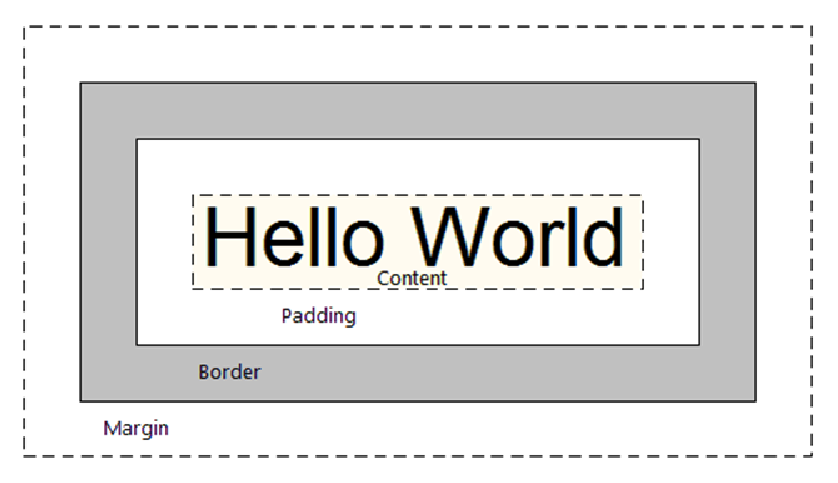
\includegraphics[scale=0.5]{box-model.eps}
	      \end{center}
	\item[$\bullet$] Vous trouverez sur le \textit{Web} des listes complètes des propriétés css, par exemple : \\ {\tt http://www.css-faciles.com/proprietes-css-liste-alphabetique.php}
\end{itemize}
\FinListe
\end{document}